% TikZ figure for tiling comparison - Non-exact tiling 1032x1032 with 43x43 base

% Define custom colors from new palette
\definecolor{gray}{HTML}{c8c8c8}
\definecolor{gold}{HTML}{f0c571}
\definecolor{teal}{HTML}{59a89c}
\definecolor{blue}{HTML}{0b81a2}
\definecolor{red}{HTML}{e25759}
\definecolor{darkred}{HTML}{9d2c00}
\definecolor{purple}{HTML}{7E4794}
\definecolor{green}{HTML}{36b700}

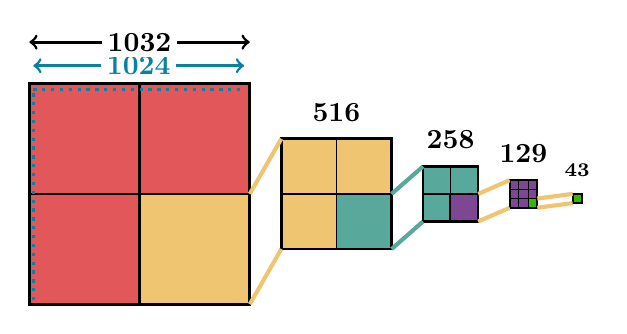
\begin{tikzpicture}[
    scale=1,
    every node/.style={font=\small},
    level1/.style={draw, line width=1.2pt, fill=blue!20},
    level2/.style={draw, line width=1.0pt, fill=green!20},
    level3/.style={draw, line width=0.8pt, fill=orange!20},
    level4/.style={draw, line width=0.6pt, fill=purple!20},
    base/.style={draw, line width=0.5pt, fill=red!30},
    popup/.style={draw, line width=2pt, fill=yellow!10, dashed},
    connector/.style={line width=1.5pt, red}
]

% Level 0: Main 1032x1032 square divided into 2x2 (4 squares of 516x516)
\begin{scope}[local bounding box=mainlevel]
    \def\mainsize{2.8}
    \def\halfsize{1.4}
    
    % Draw 2x2 grid
    \draw[draw, line width=0.8pt, fill=red] (0, 0) rectangle (\halfsize, \halfsize);
    
    \draw[draw, line width=0.8pt, fill=gold] (\halfsize, 0) rectangle (\mainsize, \halfsize);
    
    \draw[draw, line width=0.8pt, fill=red] (0, \halfsize) rectangle (\halfsize, \mainsize);
    
    \draw[draw, line width=0.8pt, fill=red] (\halfsize, \halfsize) rectangle (\mainsize, \mainsize);
    
    % Outer border
    \draw[line width=1.2pt, black] (0,0) rectangle (\mainsize, \mainsize);
    
    % Light dotted lines for 1024x1024 (exact tiling within non-exact 1032x1032) - only left and top, slightly inset
    \pgfmathsetmacro{\exactratio}{1024/1032}
    \pgfmathsetmacro{\exactsize}{\exactratio*\mainsize}
    \pgfmathsetmacro{\inset}{0.05}
    % Draw only left and top edges with small inset
    \draw[line width=1.2pt, blue, dotted] (\inset,\inset) -- (\inset, \exactsize-\inset);  % left edge
    \draw[line width=1.2pt, blue, dotted] (\inset,\exactsize-\inset) -- (\exactsize-\inset, \exactsize-\inset);  % top edge
    
    % Bidirectional arrow showing 1024 extent with label in center
    \draw[<->, line width=1pt, blue] (\inset, \exactsize-\inset+0.3) -- (\exactsize-\inset, \exactsize-\inset+0.3) node[midway, fill=white, inner sep=2pt, font=\bfseries, text=blue] {1024};
    
    % Bidirectional arrow showing 1032 extent with label in center (0.3 units above 1024 arrow)
    \draw[<->, line width=1pt, black] (0, \exactsize-\inset+0.6) -- (\mainsize, \exactsize-\inset+0.6) node[midway, fill=white, inner sep=2pt, font=\bfseries] {1032};
\end{scope}

% Level 1: Popup showing 516x516 divided into 2x2 (4 squares of 258x258)
\begin{scope}[shift={(3.2, 0.7)}, local bounding box=level1box]
    \def\popsize{1.4}
    \def\quartsize{0.7}
    
    % Draw 2x2 grid
    \draw[draw, line width=0.6pt, fill=gold] (0, 0) rectangle (\quartsize, \quartsize);
    
    \draw[draw, line width=0.6pt, fill=teal] (\quartsize, 0) rectangle (\popsize, \quartsize);
    
    \draw[draw, line width=0.6pt, fill=gold] (0, \quartsize) rectangle (\quartsize, \popsize);
    
    \draw[draw, line width=0.6pt, fill=gold] (\quartsize, \quartsize) rectangle (\popsize, \popsize);
    
    % Outer border
    \draw[line width=1.0pt, black] (0,0) rectangle (\popsize, \popsize);
    \node[above, font=\bfseries] at (\popsize/2, \popsize+0.1) {516};
\end{scope}

% Connectors from Level 0 to Level 1 (expanded 516 to entire 516 square)
\draw[connector, gold] (2.8, 1.4) -- (3.2, 2.1);  % top right to top left of entire Level 1
\draw[connector, gold] (2.8, 0) -- (3.2, 0.7);  % bottom right to bottom left of entire Level 1

% Level 2: Popup showing 258x258 divided into 2x2 (4 squares of 129x129)
\begin{scope}[shift={(5, 1.05)}, local bounding box=level2box]
    \def\popsize{0.7}
    \def\quartsize{0.35}
    
    % Draw 2x2 grid
    \draw[draw, line width=0.8pt, fill=teal] (0, 0) rectangle (\quartsize, \quartsize);
    
    \draw[draw, line width=0.6pt, fill=purple] (\quartsize, 0) rectangle (\popsize, \quartsize);
    
    \draw[draw, line width=0.6pt, fill=teal] (0, \quartsize) rectangle (\quartsize, \popsize);
    
    \draw[draw, line width=0.6pt, fill=teal] (\quartsize, \quartsize) rectangle (\popsize, \popsize);
    
    % Outer border
    \draw[line width=0.9pt, black] (0,0) rectangle (\popsize, \popsize);
    \node[above, font=\bfseries] at (\popsize/2, \popsize+0.1) {258};
\end{scope}

% Connectors from Level 1 to Level 2 (expanded 258 to entire 258 square)
\draw[connector, teal] (4.6, 1.4) -- (5, 1.75);  % top right to top left of entire Level 2
\draw[connector, teal] (4.6, 0.7) -- (5, 1.05);   % bottom right to bottom left of entire Level 2

% Level 3: Popup showing 129x129 divided into 3x3 (9 squares of 43x43)
\begin{scope}[shift={(6.1, 1.225)}, local bounding box=level3box]
    \def\gridsize{0.35}
    \def\cellsize{0.117}
    
    % Draw 3x3 grid with different colors
    \def\cellcolors{{"purple","purple","purple","purple","purple","purple","purple","purple"}}
    \pgfmathsetmacro{\colorindex}{0}
    \foreach \i in {0,1,2} {
        \foreach \j in {0,1,2} {
            \pgfmathsetmacro{\xpos}{\i*\cellsize}
            \pgfmathsetmacro{\ypos}{\j*\cellsize}
            \ifnum\i=2
                \ifnum\j=0
                    \draw[draw, line width=0.4pt, fill=green] (\xpos, \ypos) rectangle ++(\cellsize, \cellsize);
                \else
                    \pgfmathparse{\cellcolors[int(\colorindex)]}
                    \edef\currentcolor{\pgfmathresult}
                    \expandafter\draw\expandafter[draw, line width=0.4pt, fill=\currentcolor] (\xpos, \ypos) rectangle ++(\cellsize, \cellsize);
                    \pgfmathsetmacro{\colorindex}{\colorindex+1}
                    \global\let\colorindex\colorindex
                \fi
            \else
                \pgfmathparse{\cellcolors[int(\colorindex)]}
                \edef\currentcolor{\pgfmathresult}
                \expandafter\draw\expandafter[draw, line width=0.4pt, fill=\currentcolor] (\xpos, \ypos) rectangle ++(\cellsize, \cellsize);
                \pgfmathsetmacro{\colorindex}{\colorindex+1}
                \global\let\colorindex\colorindex
            \fi
        }
    }
    
    % Outer border
    \draw[line width=0.8pt, black] (0,0) rectangle (\gridsize, \gridsize);
    \node[above, font=\bfseries] at (\gridsize/2, \gridsize+0.1) {129};
\end{scope}

% Connectors from Level 2 to Level 3 (expanded 129 to entire 129 square)
\draw[connector, gold] (5.7, 1.4) -- (6.1, 1.575);  % top right to top left of entire Level 3
\draw[connector, gold] (5.7, 1.05) -- (6.1, 1.225);      % bottom right to bottom left of entire Level 3

% Level 4: Show the base multiplier with included PDF
\begin{scope}[shift={(6.9, 1.2835)}, local bounding box=level4box]
    \def\basesize{0.117}
    
    % Draw square with same color as expanded square
    \draw[draw, line width=0.7pt, black, fill=green] (0,0) rectangle (\basesize, \basesize);
    
    % Label on top
    \node[above, font=\scriptsize\bfseries] at (\basesize/2, \basesize+0.1) {43};
\end{scope}

% Connectors from Level 3 to Level 4 (expanded 43 to entire base square)
\draw[connector, gold] (6.451, 1.342) -- (6.9, 1.4005);   % top right to top left of base
\draw[connector, gold] (6.451, 1.225) -- (6.9, 1.2835); % bottom right to bottom left of base

\end{tikzpicture}
